\subsection{Incorporating E(3) Features}
\label{subsec:incorporate_e3_features}

\begin{figure*}[t]
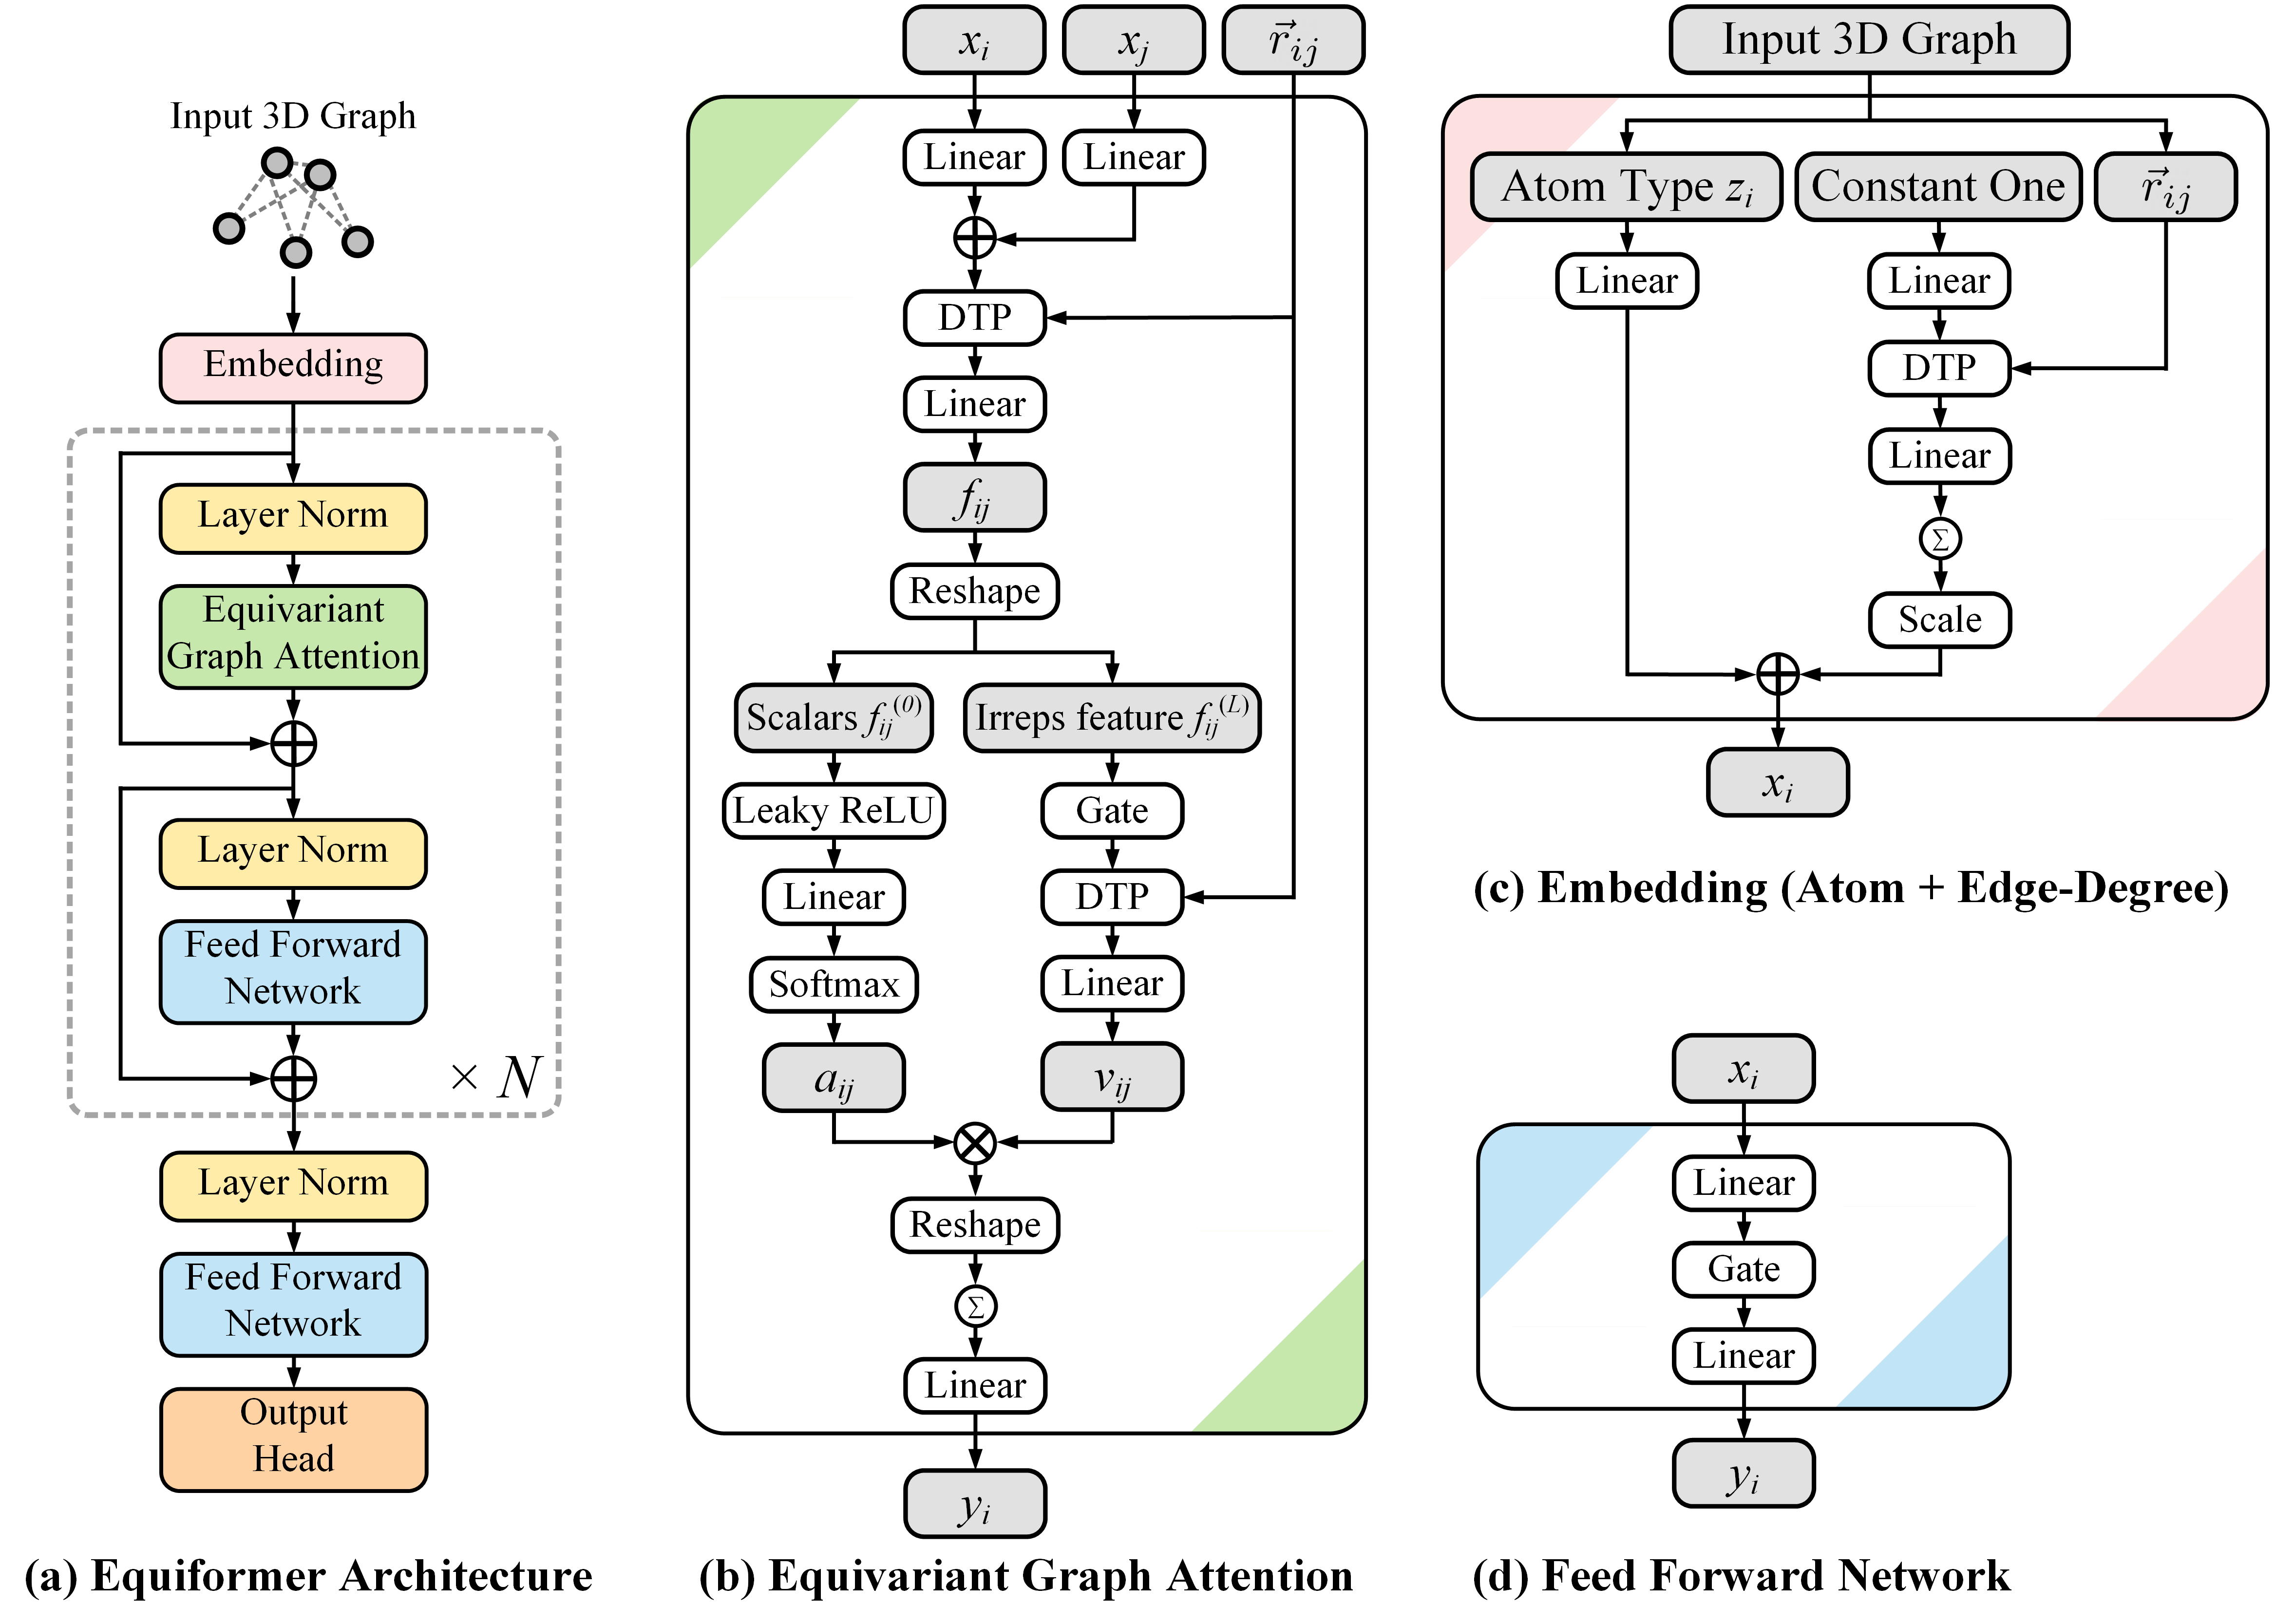
\includegraphics[width=0.9\linewidth]{figure/equiformer.png}
\centering
\caption{\textbf{Architecture of Equiformer.}
\todo{Add detailed explanation of each submodule of Attention to figures in Appendix.}
\todo{Add dot product attention in Appendix.}
\todo{Update variables: $x_{ij}, a_{ij}, v_{ij}$}
Here ``$\otimes$'' denotes multiplication, ``$\oplus$'' denotes addition, and ``DTP'' stands for depth-wise tensor product. $\sum$ within a circle denotes summation over all neighbors.
}
\label{fig:equiformer}
\end{figure*}

\begin{enumerate}
    \item \note{Typical GNN and Transformer operate on scalars}
    \item \note{Equivariance}
    \item \note{Including E(3)}
    \item \note{Picture for Linear, Gate, DTP, Layer Norm}
\end{enumerate}

\todo{May be moved to Background}

\todo{Definition of Graph and 3D Graph}


\paragraph{Directional Information.}
Typical graph neural networks (GNNs) use scalars as internal representations.
As scalars are invariant features, after geometric transformations like rotations, they will remain the same.
This means that the representations are insensitive to rotations and therefore cannot encode any directional information.
However, directional information contained in quantities like forces is indispensable to understand interactions between atoms from the perspective of physics.
Moreover, discarding directional information can make GNNs less expressive as they cannot differentiate certain types of graphs.
These motivate using other representations instead of only scalars.


\paragraph{Equivariance.}

\paragraph{E(3) Features.}
